\documentclass[border=5pt]{standalone}

\usepackage{tikz}
\usepackage{etoolbox}
\usetikzlibrary{positioning}
 \usetikzlibrary{calc} 

\pgfdeclarelayer{background}
\pgfdeclarelayer{foreground}
\pgfdeclarelayer{sankeydebug}
\pgfsetlayers{background,main,foreground,sankeydebug}

\newif\ifsankeydebug

\newenvironment{sankeydiagram}[1][]{

  \def\sankeyflow##1##2{% sn, en
    \path[sankey fill]
    let
    \p1=(##1.north east),\p2=(##1.south east),
    \n1={atan2(\y1-\y2,\x1-\x2)-90},
    \p3=(##2.north west),\p4=(##2.south west),
    \n2={atan2(\y3-\y4,\x3-\x4)+90}
    in
    (\p1) to[out=\n1,in=\n2] (\p3) --
    (\p4) to[in=\n1,out=\n2] (\p2) -- cycle;
    \draw[sankey draw]
    let
    \p1=(##1.north east),\p2=(##1.south east),
    \n1={atan2(\y1-\y2,\x1-\x2)-90},
    \p3=(##2.north west),\p4=(##2.south west),
    \n2={atan2(\y3-\y4,\x3-\x4)+90}
    in
    (\p1) to[out=\n1,in=\n2] (\p3)
    (\p4) to[in=\n1,out=\n2] (\p2);
  }


  \tikzset{
    sankey tot length/.store in=\sankeytotallen,
    sankey tot quantity/.store in=\sankeytotalqty,
    sankey min radius/.store in=\sankeyminradius,
    sankey arrow length/.store in=\sankeyarrowlen,
    sankey debug/.is if=sankeydebug,
    sankey debug=false,
    sankey flow/.style={
      to path={
        \pgfextra{
          \pgfinterruptpath
          \edef\sankeystart{\tikztostart}
          \edef\sankeytarget{\tikztotarget}
          \sankeyflow{\sankeystart}{\sankeytarget}
          \endpgfinterruptpath
        }
      },
    },
    sankey node/.style={
      inner sep=0,minimum height={sankeyqtytolen(##1)},
      minimum width=0,draw=none,line width=0pt,
    },
    % sankey angle
    sankey angle/.store in=\sankeyangle,
    % sankey default styles
    sankey fill/.style={line width=0pt,fill,white},
    sankey draw/.style={draw=black,line width=.4pt},
  }

  \newcommand\sankeynode[4]{%prop,orientation,name,pos
    \node[sankey node=##1,rotate=##2] (##3) at (##4) {};
    \ifsankeydebug
    \begin{pgfonlayer}{sankeydebug}
      \draw[red,|-|] (##3.north west) -- (##3.south west);
      \pgfmathsetmacro{\len}{sankeyqtytolen(##1)/3}
      \draw[red] (##3.west)
      -- ($(##3.west)!\len pt!90:(##3.south west)$)
      node[font=\tiny,text=black] {##3};
    \end{pgfonlayer}
    \fi
  }

  \newcommand\sankeynodestart[4]{%prop,orientation,name,pos
    \sankeynode{##1}{##2}{##3}{##4}
    \begin{scope}[shift={(##3)},rotate=##2]
      \path[sankey fill]
      (##3.north west) -- ++(-\sankeyarrowlen,0)
      -- ([xshift=-\sankeyarrowlen/6]##3.west)
      -- ([xshift=-\sankeyarrowlen]##3.south west)
      -- (##3.south west) -- cycle;
      \path[sankey draw]
      (##3.north west) -- ++(-\sankeyarrowlen,0)
      -- ([xshift=-\sankeyarrowlen/6]##3.west)
      -- ([xshift=-\sankeyarrowlen]##3.south west)
      -- (##3.south west);
    \end{scope}
  }

  \newcommand\sankeynodeend[4]{%prop,orientation,name,pos
    \sankeynode{##1}{##2}{##3}{##4}
    \begin{scope}[shift={(##3)},rotate=##2]
      \path[sankey fill]
      (##3.north east)
      -- ([xshift=\sankeyarrowlen]##3.east)
      -- (##3.south west) -- cycle;
      \path[sankey draw]
      (##3.north east)
      -- ([xshift=\sankeyarrowlen]##3.east)
      -- (##3.south west);
    \end{scope}
  }

  \newcommand\sankeyadvance[3][]{%newname,name,distance
    \edef\name{##2}
    \ifstrempty{##1}{
      \def\newname{##2}
      \edef\name{##2-old}
      \path [late options={name=##2,alias=\name}];
    }{
      \def\newname{##1}
    }
    \path
    let
    % sankey node angle
    \p1=(##2.north east),
    \p2=(##2.south east),
    \n1={atan2(\y1-\y2,\x1-\x2)-90},
    % sankey prop
    \p3=($(\p1)-(\p2)$),
    \n2={sankeylentoqty(veclen(\x3,\y3))},
    % next position
    \p4=($(##2.east)!##3!-90:(##2.north east)$)
    in
    \pgfextra{
      \pgfmathsetmacro{\prop}{\n2}
      \pgfinterruptpath
      \sankeynode{\prop}{\n1}{\newname}{\p4}
      \path (\name) to[sankey flow] (\newname);
      \endpgfinterruptpath
    };
  }

  \newcommand\sankeyturn[3][]{%newname,name,angle
    \edef\name{##2}
    \ifstrempty{##1}{
      \def\newname{##2}
      \edef\name{##2-old}
      \path [late options={name=##2,alias=\name}];
    }{
      \def\newname{##1}
    }
    \ifnumgreater{##3}{0}{
      \typeout{turn acw: ##3}
      \path
      let
      % sankey node angle
      \p1=(##2.north east),
      \p2=(##2.south east),
      \p3=($(\p1)!-\sankeyminradius!(\p2)$),
      \n1={atan2(\y1-\y2,\x1-\x2)-90},
      % sankey prop
      \p4=($(\p1)-(\p2)$),
      \n2={sankeylentoqty(veclen(\x4,\y4))},
      \p5=(##2.east),
      \p6=($(\p3)!1!##3:(\p5)$)
      in
      \pgfextra{
        \pgfmathsetmacro{\prop}{\n2}
        \pgfinterruptpath
        % \fill[red] (\p3) circle (2pt);
        % \fill[blue](\p6) circle (2pt);
        \sankeynode{\prop}{\n1+##3}{\newname}{\p6}
        \path (\name) to[sankey flow] (\newname);
        \endpgfinterruptpath
      };
    }{
      \typeout{turn acw: ##3}
      \path
      let
      % sankey node angle
      \p1=(##2.south east),
      \p2=(##2.north east),
      \p3=($(\p1)!-\sankeyminradius!(\p2)$),
      \n1={atan2(\y1-\y2,\x1-\x2)+90},
      % sankey prop
      \p4=($(\p1)-(\p2)$),
      \n2={sankeylentoqty(veclen(\x4,\y4))},
      \p5=(##2.east),
      \p6=($(\p3)!1!##3:(\p5)$)
      in
      \pgfextra{
        \pgfmathsetmacro{\prop}{\n2}
        \pgfinterruptpath
        % \fill[red] (\p3) circle (2pt);
        % \fill[blue](\p6) circle (2pt);
        \sankeynode{\prop}{\n1+##3}{\newname}{\p6}
        \path (\name) to[sankey flow] (\newname);
        \endpgfinterruptpath
      };
    }
  }

  \newcommand\sankeyfork[2]{%name,list of forks
    \def\name{##1}
    \def\listofforks{##2}
    \xdef\sankeytot{0}
    \path 
    let
    % sankey node angle
    \p1=(\name.north east),
    \p2=(\name.south east),
    \n1={atan2(\y1-\y2,\x1-\x2)-90},
    % sankey prop
    \p4=($(\p1)-(\p2)$),
    \n2={sankeylentoqty(veclen(\x4,\y4))}
    in
    \pgfextra{
      \pgfmathsetmacro{\iprop}{\n2}
    }
    \foreach \prop/\name[count=\c] in \listofforks {
      let
      \p{start \name}=($(\p1)!\sankeytot/\iprop!(\p2)$),
      \n{nexttot}={\sankeytot+\prop},
      \p{end \name}=($(\p1)!\n{nexttot}/\iprop!(\p2)$),
      \p{mid \name}=($(\p{start \name})!.5!(\p{end \name})$)
      in
      \pgfextra{
        \xdef\sankeytot{\n{nexttot}}
        \pgfinterruptpath
        \sankeynode{\prop}{\n1}{\name}{\p{mid \name}}
        \endpgfinterruptpath
      }
    }
    \pgfextra{
      \pgfmathsetmacro{\diff}{abs(\iprop-\sankeytot)}
      \pgfmathtruncatemacro{\finish}{\diff<0.01?1:0}
      \ifnumequal{\finish}{1}{}{
        \message{*** Warning: bad sankey fork (maybe)...}
        \message{\iprop-\sankeytot}
      }
    };
  }

  \tikzset{
    % default values,
    declare function={
      sankeyqtytolen(\qty)=\qty/\sankeytotalqty*\sankeytotallen;
      sankeylentoqty(\len)=\len/\sankeytotallen*\sankeytotalqty;
    },
    sankey tot length=100pt,
    sankey tot quantity=100,
    sankey min radius=30pt,%
    sankey arrow length=10pt,%
    % user values
    #1}
}{
}


\begin{document}
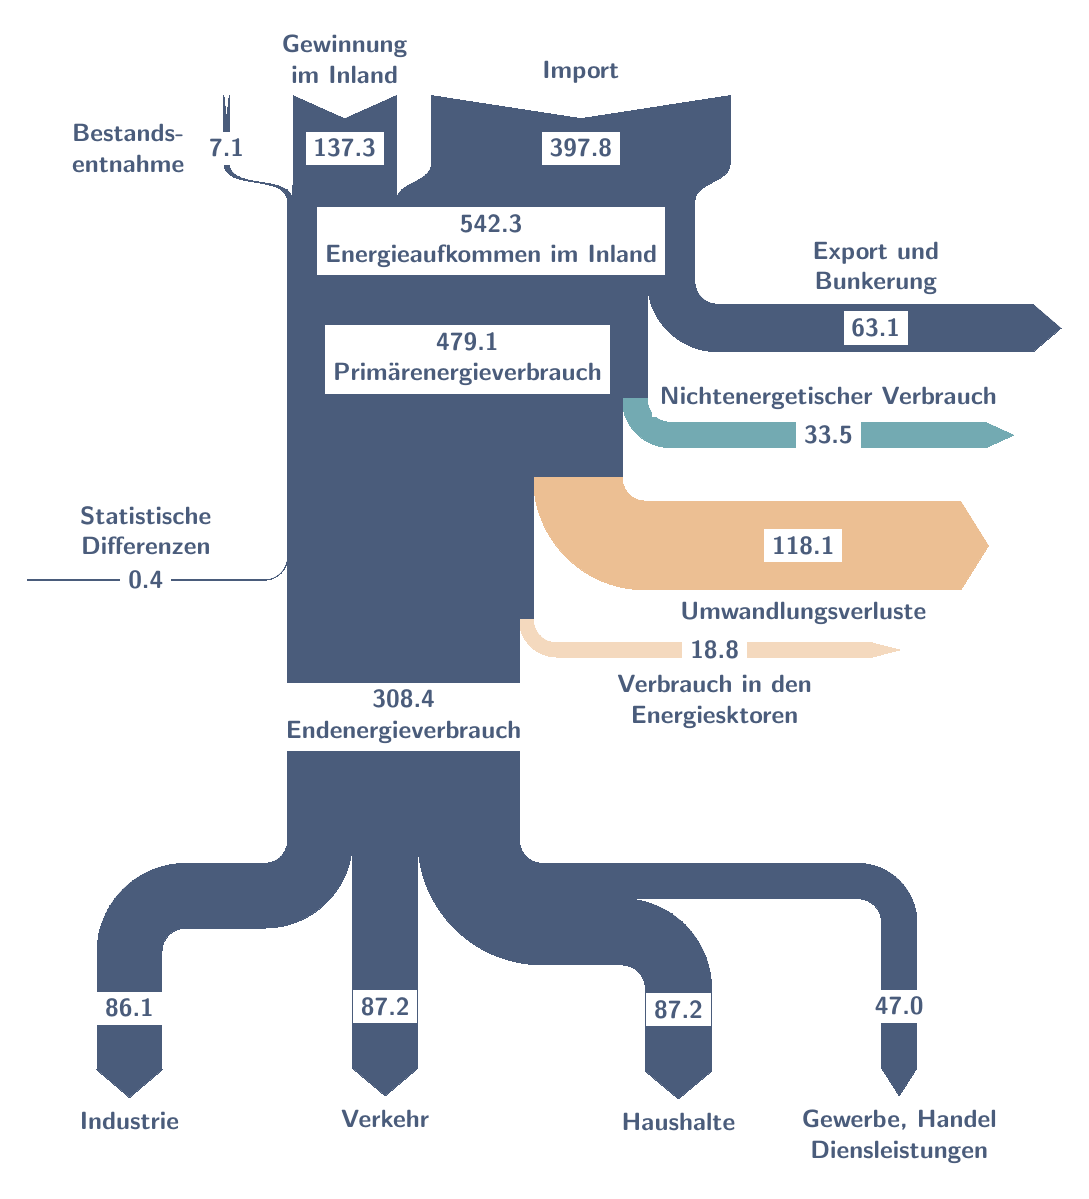
\begin{tikzpicture}

  \begin{sankeydiagram}[
    sankey tot length=5cm,%
    sankey tot quantity=524.3,%
    sankey min radius=3mm,%
    sankey fill/.style={
      draw,line width=0pt,
      fill,
      cyan!50!blue!50!black,
    },
    sankey draw/.style={
      draw=none,
      line width=1pt,
      line cap=round,
      line join=round,
    },
    %sankey debug,
    ]

    \sankeynodestart{7.2}{-90}{B}{-.5,0}
    \coordinate[below=1mm of B.center] (B label);
    \sankeyadvance{B}{5mm}
    \sankeynodestart{137.3}{-90}{GI}{1,0}
    \coordinate[below=1mm of GI.center] (GI label);
    \sankeyadvance{GI}{5mm}
    \sankeynodestart{397.8}{-90}{I}{4,0}
    \coordinate[below=1mm of I.center] (I label);
    \sankeyadvance{I}{5mm}

    \sankeynode{542.3}{-90}{EI}{2.86,-1}
    \sankeyfork{EI}{397.8/Ia,137.3/GIa,7.2/Ba}
    \path (I) to[sankey flow] (Ia);
    \path (GI) to[sankey flow] (GIa);
    \path (B) to[sankey flow] (Ba);
    \sankeyadvance{EI}{5mm}
    \coordinate (EI label) at (EI);
    \sankeyadvance{EI}{5mm}

    \sankeyfork{EI}{63.1/EB,479.2/P}

    \sankeyturn{EB}{90}
    \sankeyadvance{EB}{2cm}
    \coordinate (EB label) at (EB.center);
    \sankeyadvance{EB}{2cm}
    \sankeynodeend{63.1}{0}{EB}{EB}

    \sankeyadvance{P}{10mm}
    \coordinate (P label) at (P);
    \sankeyadvance{P}{5mm}

    \sankeyfork{P}{33.5/NV,445.7/P}

    {
      \tikzset{sankey fill/.append style={cyan!80!lime!50!gray}}
      \sankeyturn{NV}{90}
      \sankeyadvance{NV}{2cm}
      \coordinate (NV label) at (NV);
      \sankeyadvance{NV}{2cm}
      \sankeynodeend{33.5}{0}{NV}{NV}
    }

    \sankeyadvance{P}{10mm}

    \sankeyfork{P}{118.1/U,327.6/P}

    {
      \tikzset{sankey fill/.append style={orange!70!gray!50}}
      \sankeyturn{U}{90}
      \sankeyadvance{U}{2cm}
      \coordinate (U label) at (U);
      \sankeyadvance{U}{2cm}
      \sankeynodeend{118.1}{0}{U}{U}
    }

    \sankeyadvance{P}{10mm}

    \sankeyfork{P}{327.2/P,0.4/SD}

    {
      \sankeyturn{SD}{-90}
      \sankeyadvance{SD}{15mm}
      \coordinate (SD label) at (SD);
      \sankeyadvance{SD}{15mm}
      \sankeynodeend{0.4}{0}{SD}{SD}
    }

    \sankeyadvance{P}{8mm}

    \sankeyfork{P}{18.8/VE,308.4/E}

    {
      \tikzset{sankey fill/.append style={orange!70!gray!30}}
      \sankeyturn{VE}{90}
      \sankeyadvance{VE}{2cm}
      \coordinate (VE label) at (VE);
      \sankeyadvance{VE}{2cm}
      \sankeynodeend{18.8}{0}{VE}{VE}
    }

    \sankeyadvance{E}{8mm}
    \coordinate (E label) at (E);
    \sankeyadvance{E}{20mm}

    \sankeyfork{E}{135.1/H+GHD,87.2/V,86.1/In}

    \sankeyturn{In}{-90}
    \sankeyadvance{In}{10mm}
    \sankeyturn{In}{90}
    \sankeyadvance{In}{5mm}
    \coordinate (In label)  at (In);
    \sankeyadvance{In}{10mm}
    \sankeynodeend{86.7}{-90}{In}{In}

    \sankeyadvance{V}{19mm}
    \coordinate (V label) at (V);
    \sankeyadvance{V}{10mm}
    \sankeynodeend{87.2}{-90}{V}{V}

    \sankeyturn{H+GHD}{90}
    \sankeyadvance{H+GHD}{10mm}
    \sankeyfork{H+GHD}{47.0/GHD,88.1/H}

    \sankeyturn{H}{-90}
    \sankeyadvance{H}{.5mm}
    \coordinate (H label) at (H);
    \sankeyadvance{H}{10mm}
    \sankeynodeend{88.1}{-90}{H}{H}

    \sankeyadvance{GHD}{30mm}
    \sankeyturn{GHD}{-90}
    \sankeyadvance{GHD}{8.5mm}
    \coordinate (GHD label) at (GHD);
    \sankeyadvance{GHD}{10mm}
    \sankeynodeend{47}{-90}{GHD}{GHD}



    % labels
    \tikzset{
      label/.style={
        fill=white,inner sep=.5mm,text=cyan!50!blue!50!black,
        font=\sffamily\bfseries\small,inner sep=1mm,
        align=center,
      },
    }
    \node[label,anchor=north] (B label) at (B label) {7.1};
    \node[label,left=1mm of B label] {Bestands-\\entnahme};
    \node[label,anchor=north] at (GI label) {137.3};
    \node[label,above=5mm of GI label] {Gewinnung\\im Inland};
    \node[label,anchor=north] at (I label) {397.8};
    \node[label,above=5mm of I label] {Import};

    \node[label] at (EI label) {542.3\\Energieaufkommen im Inland};

    \node[label,anchor=center] (EB label) at (EB label) {63.1};
    \node[label,above=1mm of EB label] {Export und\\Bunkerung};

    \node[label] at (P label) {479.1\\Primärenergieverbrauch};

    \node[label,anchor=center] (NV label) at (NV label) {33.5};
    \node[label,above=0mm of NV label] {Nichtenergetischer Verbrauch};

    \node[label,anchor=center] (U label) at (U label) {118.1};
    \node[label,below=4mm of U label] {Umwandlungsverluste};

    \node[label,anchor=center] (SD label) at (SD label) {0.4};
    \node[label,above=0mm of SD label] {Statistische\\Differenzen};

    \node[label,anchor=center] (VE label) at (VE label) {18.8};
    \node[label,below=0mm of VE label] {Verbrauch in den\\Energiesktoren};

    \node[label,anchor=north] (E label) at (E label) {308.4\\Endenergieverbrauch};

    \node[label,anchor=north] (In label) at (In label) {86.1};
    \node[label,anchor=north,below=1cm of In label] {Industrie};

    \node[label,anchor=north] (V label) at (V label) {87.2};
    \node[label,anchor=north,below=1cm of V label] {Verkehr};

    \node[label,anchor=north] (H label) at (H label) {87.2};
    \node[label,anchor=north,below=1cm of H label] {Haushalte};

    \node[label,anchor=north] (GHD label) at (GHD label) {47.0};
    \node[label,anchor=north,below=1cm of GHD label] {Gewerbe, Handel\\Diensleistungen};
 \end{sankeydiagram}
\end{tikzpicture}
\end{document}
